% vim: spell:spelllang=en:
\documentclass[12pt, oneside]{article}
\usepackage[a4paper, left=2.5cm, right=2.5cm, top=2.5cm, bottom=2.5cm]{geometry}

\usepackage[utf8]{inputenc} % Use unicode
\usepackage[T1]{fontenc}
\usepackage[catalan]{babel} % Names in spanish

%% Bibliography:
%\usepackage{comment}
%\usepackage[
    %backend=biber,
    %style=numeric,
%]{biblatex}
%\DeclareNameAlias{default}{last-first}

%\usepackage{csquotes}       % For bibliography quotations
%\DeclareQuoteAlias{spanish}{catalan}

%\addbibresource{biblio.bib}
%% see:
%% https://www.sharelatex.com/learn/Bibliography_management_in_LaTeX#The_bibliography_file

%\usepackage{datetime} % Customize date
%% \monthyeardate\today gives the date without the day
%\newdateformat{monthyeardate}{%
    %\monthname[\THEMONTH], \THEYEAR}

% For cross references
\usepackage[colorlinks = true]{hyperref}
\usepackage[catalan]{varioref}
%\usepackage{cleveref}
%hyperref configuration so that it doesn't contrast so much colorlinks,
\hypersetup{
   linkcolor={black},
   citecolor={black},
   %linkcolor={red!50!black},
   %citecolor={blue!50!black},
   urlcolor={blue!80!black}
}

\usepackage{mathtools}  % amsmath + more
\usepackage{amsthm}     % Theorem enviroment
\usepackage{amssymb}    % More symbols
\usepackage{amstext}    % Text inside mathenv

\usepackage{relsize}    % Bigger math with mathlarger{___}
\usepackage{nicefrac}   % nice fractions in one line

\usepackage[export]{adjustbox}  % Adjust table size
\usepackage{float}              % Force tables and images position (H and H!)
\usepackage{wrapfig}            % Wrap images like in HTML

\usepackage{tabularx, colortbl, booktabs}    % Better tables
\usepackage{longtable}                      % Multiple page table

% Split cell in lines and more formating options inside table
\usepackage{array, multirow, multicol, makecell}

%\usepackage{subcaption}                     % Subfigures
%\usepackage[framemethod=tikz]{mdframed}     % Custom frames

%\usepackage[bottom]{footmisc} % Footnotes at bottom of page

%\usepackage[alsoload=hep]{siunitx}          % SI units and uncertainties
%\sisetup{locale = FR}                       % Commas and so on for spanish
%\sisetup{separate-uncertainty=true}
%\sisetup{
  %per-mode=fraction,
  %fraction-function=\nicefrac
%}

%\usepackage{tikz}
%%\usetikzlibrary{arrows}
%%\usetikzlibrary{scopes}
%\usetikzlibrary{babel}

%\usepackage{listings}       % For code blocks

%% Custom code highlight
%\definecolor{codegreen}{rgb}{0,0.6,0}
%\definecolor{codegray}{rgb}{0.5,0.5,0.5}
%\definecolor{codepurple}{rgb}{0.58,0,0.82}
%\definecolor{backcolour}{rgb}{0.95,0.95,0.92}
%\definecolor{lightblue}{RGB}{135,206,250}

%\lstdefinestyle{mystyle}{ backgroundcolor=\color{backcolour},
    %commentstyle=\color{codegreen}, keywordstyle=\color{blue},
    %numberstyle=\tiny\color{codegray}, stringstyle=\color{red},
    %identifierstyle=\color{black}, basicstyle=\footnotesize,
    %%breakatwhitespace=false,
    %breaklines=true,
    %%captionpos=b,                    keepspaces=true,
    %numbers=left,                    numbersep=5pt,
    %showspaces=false,
    %%showstringspaces=false, showtabs=false,
    %tabsize=4
%}
%\lstset{style=mystyle}

\newcommand{\whitepage}{
    \clearpage\thispagestyle{empty}\addtocounter{page}{-1} \newpage \clearpage
}

% Add command before appendix session for page numbering: A-1
%\newcommand{\appendixpagenumbering}{
    %\break
    %\pagenumbering{arabic}
    %\renewcommand{\thepage}{\thesection-\arabic{page}}
%}

%% Custom Math operators (functions not in italic in math mode):
%\DeclareMathOperator{\arcsec}{arcsec}
%\DeclareMathOperator{\arccot}{arccot}
%\DeclareMathOperator{\arccsc}{arccsc}
%\DeclareMathOperator{\cis}{cis}


\renewcommand\theadfont{\bfseries}

\title{
    PAR Laboratory Assignment\\
    Lab 1: Experimental setup and tools
}

\author{
    par2109:
    Aleix Boné,
    Alex Herrero
}

\date{
    Spring 2019-20
}

\begin{document}

%After the last session for this laboratory assignment, and before starting the
%next one, you will have to deliver a report in PDF format (other formats will
%not be accepted) describing the results and conclusions that you have obtained
%when doing the assignment. As part of the document, you will have to include
%any code fragment, figure or plot you need to support your explanations. Your
%professor will open the assignment at the Raco website and set the appropriate
%delivery dates for the delivery. Only one file has to be submitted per group
%through the Raco website.
%
%Important: In the front cover of the document, please clearly state the name of
%all components of the group, the identifier of the group (username parXXYY),
%title of the assignment, date, academic

\maketitle

\section{Node architecture and memory}%
\label{sec:node_architecture_and_memory}

%Describe the architecture of the boada server. To accompany your description,
%you should refer to the following table summarising the relevant architectural
%characteristics of the different node types available:

\begin{table}[htpb]%
    \label{tab:node_arch_and_mem}
    \centering
    %\caption{caption}
    \begin{tabular}{lccc}

    \toprule
        & \texttt{boada-1 to boada-4} & \texttt{boada-5} & \texttt{boada-6 to boada-8} \\
    \midrule
        Number of sockets per node          & 2        & 2        & 2        \\
        Number of cores per socket          & 6        & 6        & 8        \\
        Number of threads per core          & 2        & 2        & 1        \\
        Maximum core frequency              & 2395 MHz & 2600 MHz & 1700 MHz \\
    \addlinespace[1em]
        L1-I cache size (per-core)          & 32K      & 32K      & 32K      \\
        L1-D cache size (per-core)          & 32K      & 32K      & 32K      \\
        L2 cache size (per-core)            & 256K     & 256K     & 256K     \\
        Last-level cache size (per-socket)  & 12288K   & 15360K   & 20480K   \\
    \addlinespace[1em]
        Main memory size (per socket)       & 12 Gb    & 31 Gb    & 16 Gb    \\
        Main memory size (per node)         & 23 Gb    & 63 Gb    & 31 Gb    \\
    \bottomrule

    \end{tabular}
\end{table}

%Also include in the description the architectural diagram for one of the nodes
%boada-1 to boada-4 as obtained when using the lstopo command. Appropriately
%comment whatever you consider appropriate.

\begin{figure}%
    \caption{Architectural diagram for \texttt{boada-1}}%
    \label{fig:arch_boada1}
    \centering
    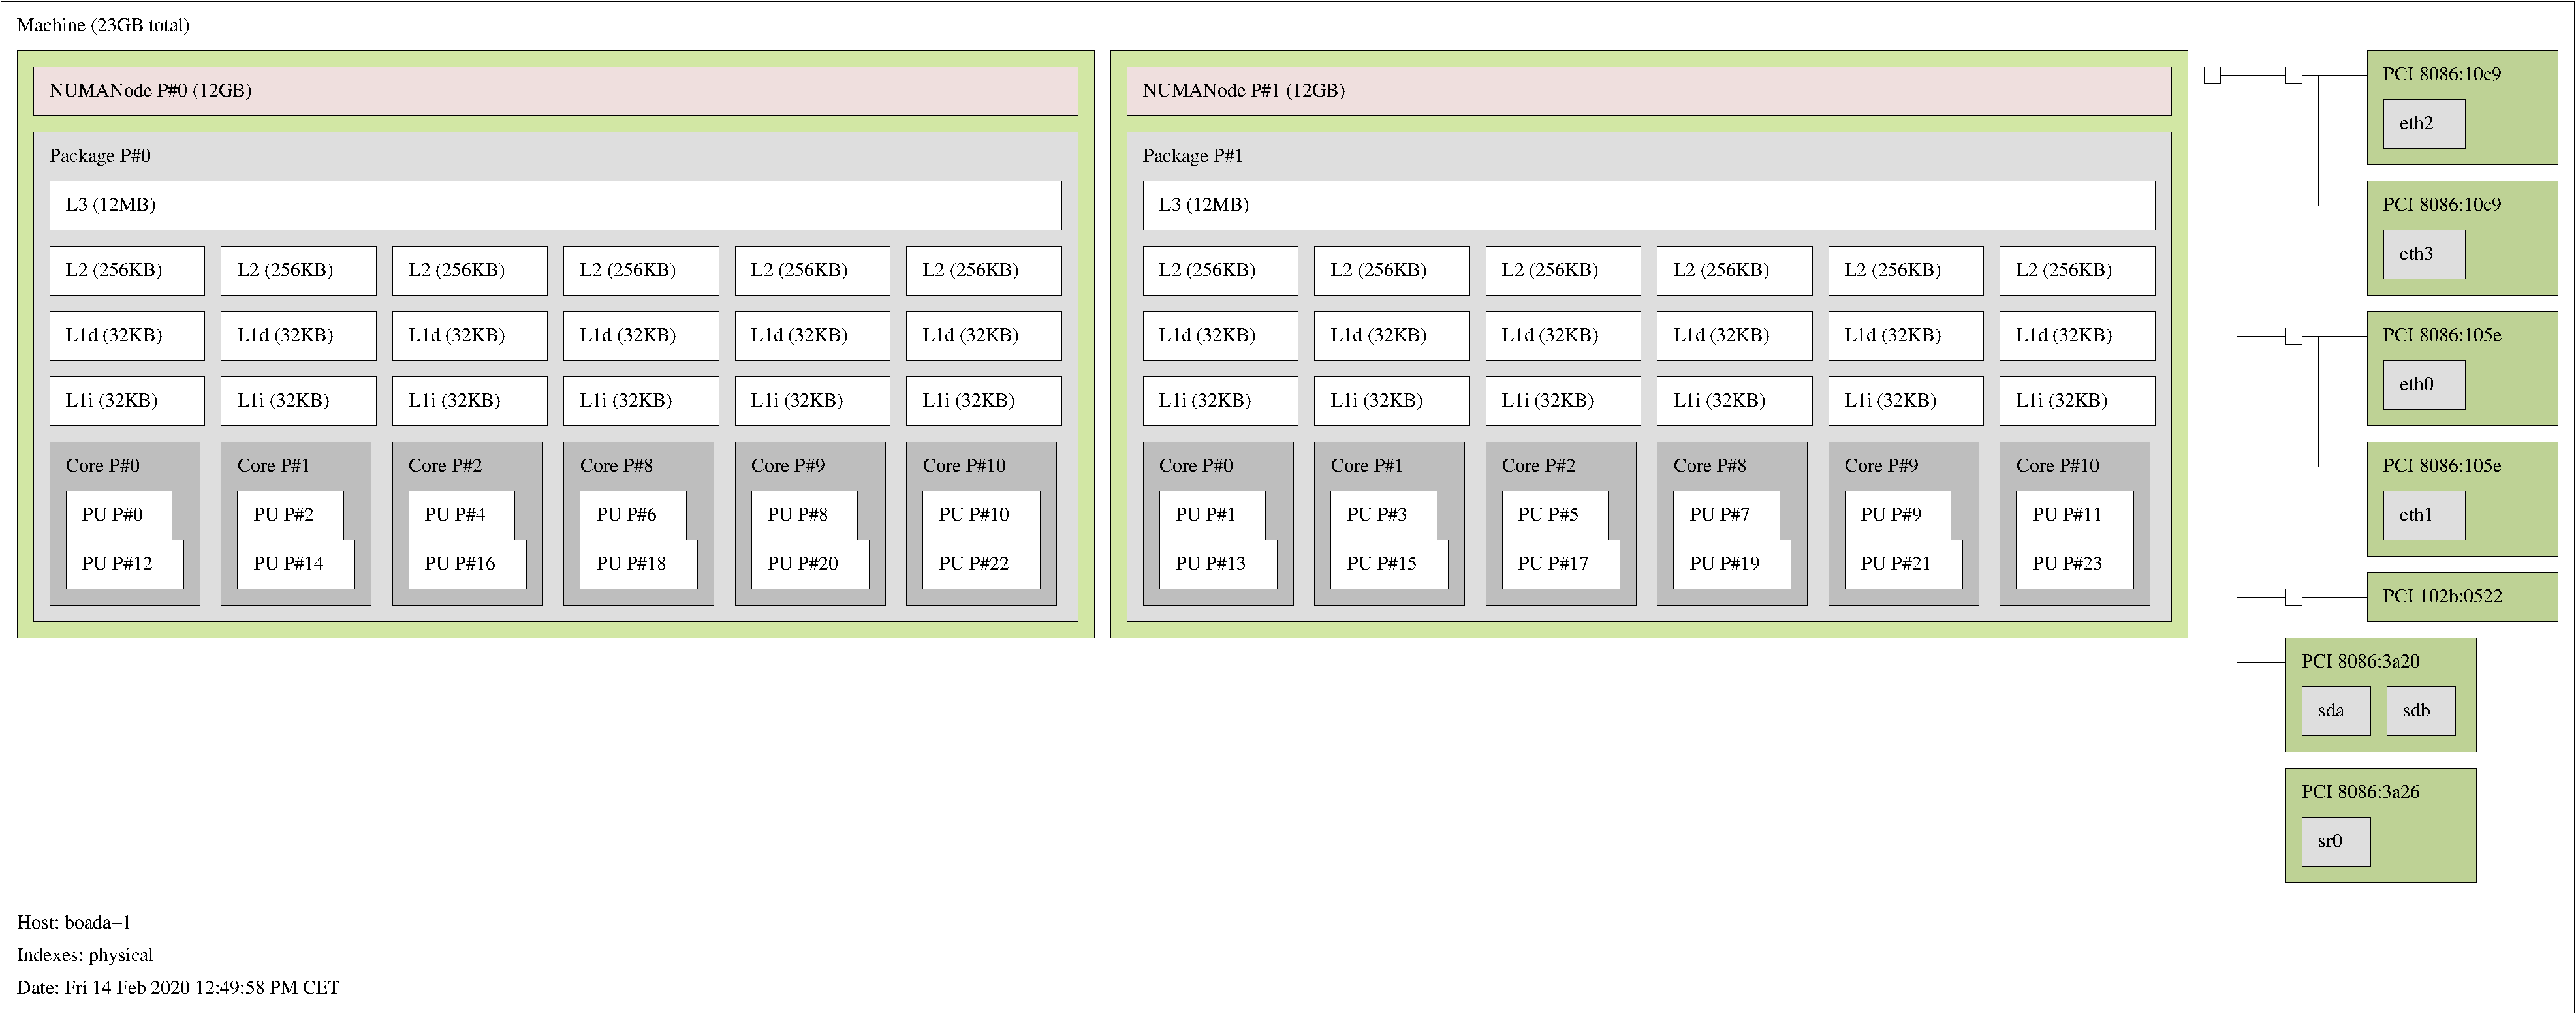
\includegraphics[width=\textwidth]{./data/map-boada-1.pdf}
\end{figure}

%TODO

\section{Strong vs.\ weak scalability}%
\label{sec:strong_vs_weak_scalability}

\begin{figure}%
    \caption{Strong scalability}%
    \label{fig:strong}
    \centering
    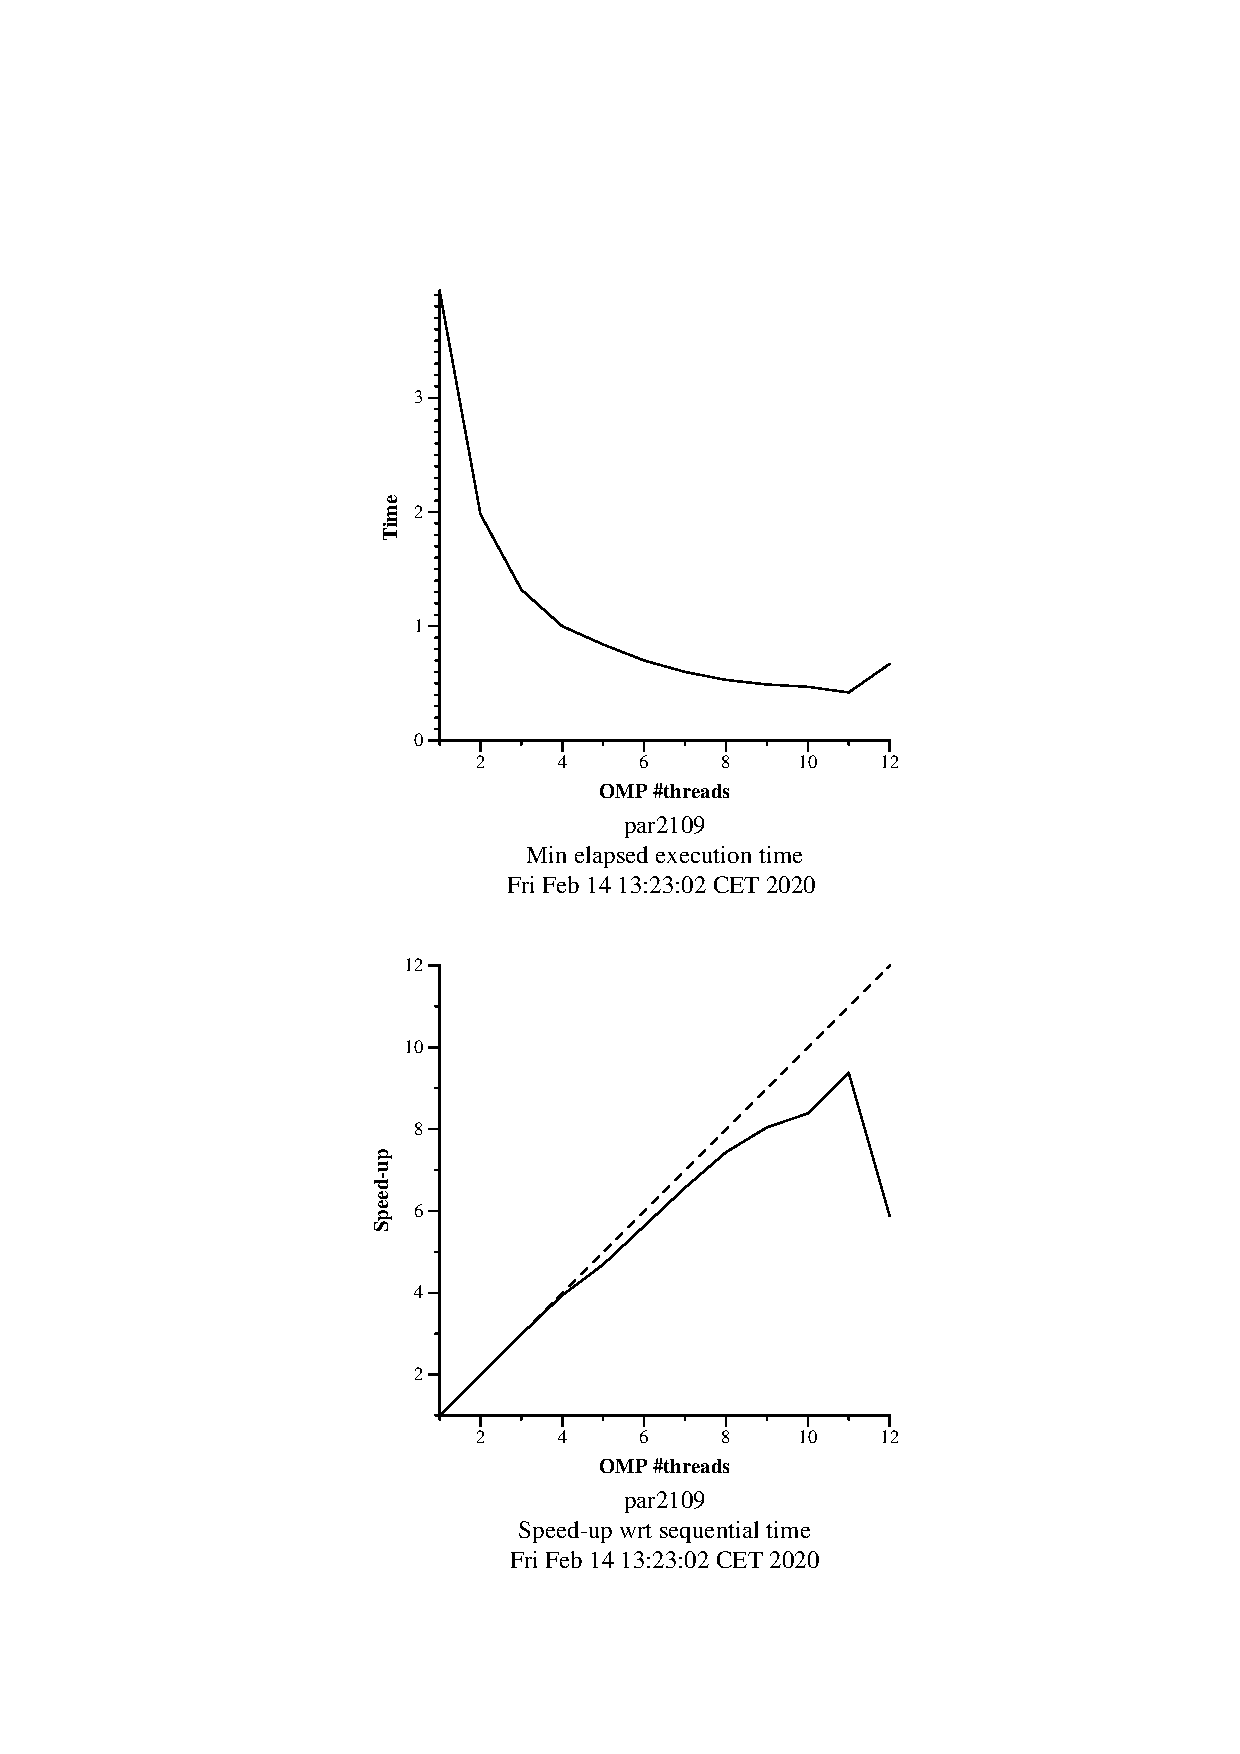
\includegraphics[width=\textwidth]{./data/pi/pi_omp-1000000000-1-12-3-strong-boada-2.pdf}
\end{figure}


\begin{figure}%
    \caption{Weak scalability}%
    \label{fig:weak}
    \centering
    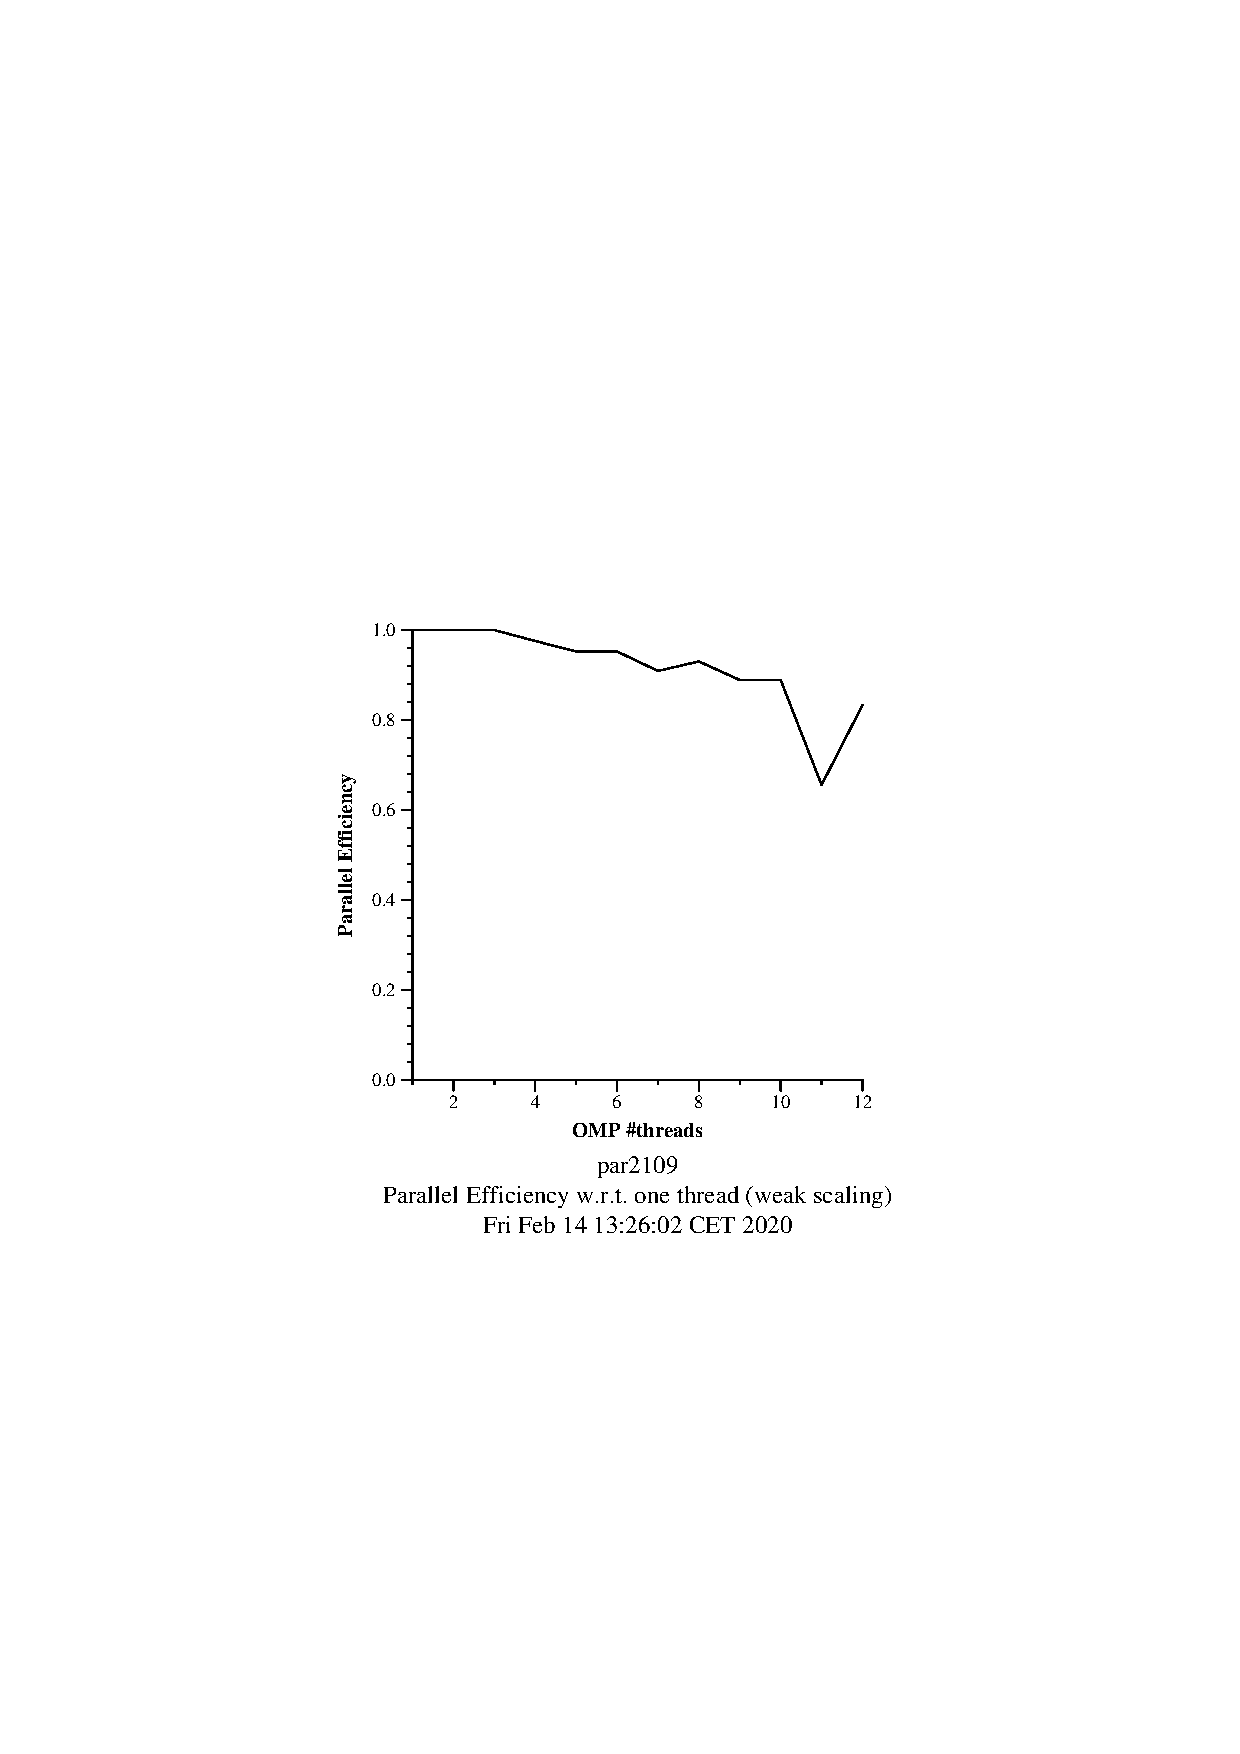
\includegraphics[width=\textwidth]{./data/pi/pi_omp-100000000-1-12-3-weak-boada-3.pdf}
\end{figure}
%Briefly explain what strong and weak scalability refer to. Exemplify your
%explanation using the execution time and speed–up plots that you obtained for
%pi omp.c. Reason about the results obtained.

\section{Analysis of task decompositions for \emph{3DFFT}}%
\label{sec:analysis_of_task_decompositions_for_3dfft}

%In this part of the report you should summarise the main conclusions from the
%analysis of task decompositions for the 3DFFT program. Backup your conclusions
%with the following table properly filled in with the information obtained in
%the laboratory session for the initial and different versions generated

\begin{table}[htpb]%
    \label{tab:parallelism}
    \centering
    %\caption{caption}
    \begin{tabular}{cccc}
    \toprule
    \thead{Version} & $T_1$ & $T_\infty$ & \thead{Parallelism} \\
    \midrule
    seq     & a & b & c \\
    v1      & a & b & c \\
    v2      & a & b & c \\
    v3      & a & b & c \\
    v4      & a & b & c \\
    v5      & a & b & c \\
    \bottomrule
    \end{tabular}
\end{table}

%For versions v4 and v5 of 3dfft tar.c perform an analysis of the potential
%strong scalability that is expected. For that include a plot with the
%execution time and/or speedup when using 1, 2, 4, 8, 16 and 32 processors, as
%reported by the simulation module inside Tareador. You should also include the
%relevant(s) part(s) of the code that help the reader to understand why v5 is
%able to scale to a higher number of processors compared to v4, capturing the
%task dependence graphs that are obtained with

\begin{figure}%
    \caption{Execution time of v5 with 1 processor}%
    \label{fig:plot_v5_01}
    \centering
    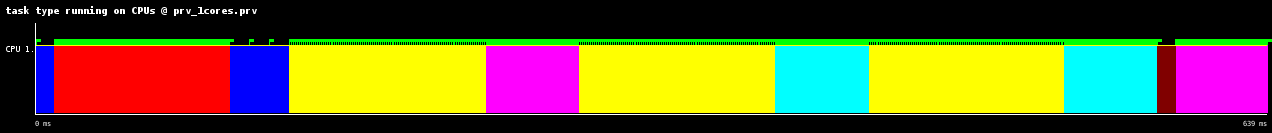
\includegraphics[width=\textwidth]{./data/3dfft/plots/v5_01.png}
\end{figure}

\begin{figure}%
    \caption{Execution time of v5 with 2 processor}%
    \label{fig:plot_v5_02}
    \centering
    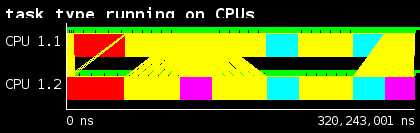
\includegraphics[width=\textwidth]{./data/3dfft/plots/v5_02.png}
\end{figure}

\section{Understanding the parallel execution of \emph{3DFFT}}%
\label{sec:understanding_the_parallel_execution_of_3dfft}

%In this final section of your report you should comment about how did you
%observed with Paraver the parallel performance evolution for the OpenMP
%parallel versions of 3DFFT. Support your explanations with the results reported
%in the following table which you obtained during the laboratory session. It is
%very important that you include the relevant Paraver captures (timelines and
%profiles of the % of time

\begin{table}[htpb]%
    \label{tab:under_parallelism}
    \centering
    %\caption{caption}
    \begin{tabular}{lcc@{\hskip 2em}ccc}
    \toprule
    \thead{Version} & $\phi$ & $S_\infty$ & $T_1$ & $T_8$ & $S_8$ \\
    \midrule
    initial version in \texttt{3dfft\_omp.c}                & 0.5692 & 2.3211 & 2382.891 ms & 1.469 ms & 1621.58 \\
    new version with improved $\phi$                        & phi & Sinf & t1 & t8 & S8 \\
    final version\footnote{with reduced parallelization overheads}    & phi & Sinf & t1 & t8 & S8 \\
    \bottomrule
    \end{tabular}
\end{table}

%Finally you should comment about the (strong) scalability plots (execution time
%and speed–up) that are obtained when varying the number of threads for the
%three parallel versions that you have analysed.

\end{document}
